\section{Accuracy}\label{section:accuracy}

One of the essential evaluation metrics is the algorithm's accuracy, which will be measured in this section. In the beginning, the approaches presented in sections \ref{section:hierarchical} and \ref{section:2stage} will be compared using PR curves in all three environments. Afterward, the best thresholds will be picked, and the final accuracy measured for both approaches and compared with the accuracy of the visual matching used in the OpenRatSLAM.\par
The thresholds are one of the factors that influence the results the most. To find the best threshold values and to adequately compare both techniques, the accuracy, recall, and precision were measured for all possible threshold combinations with 0.01 steps. The measured values for all different thresholds were used to build the PR curves, presented in Figure \ref{fig:prCurves}.\par

\begin{figure}[!tbp]
    \centering
    \subfloat[Warehouse environment]{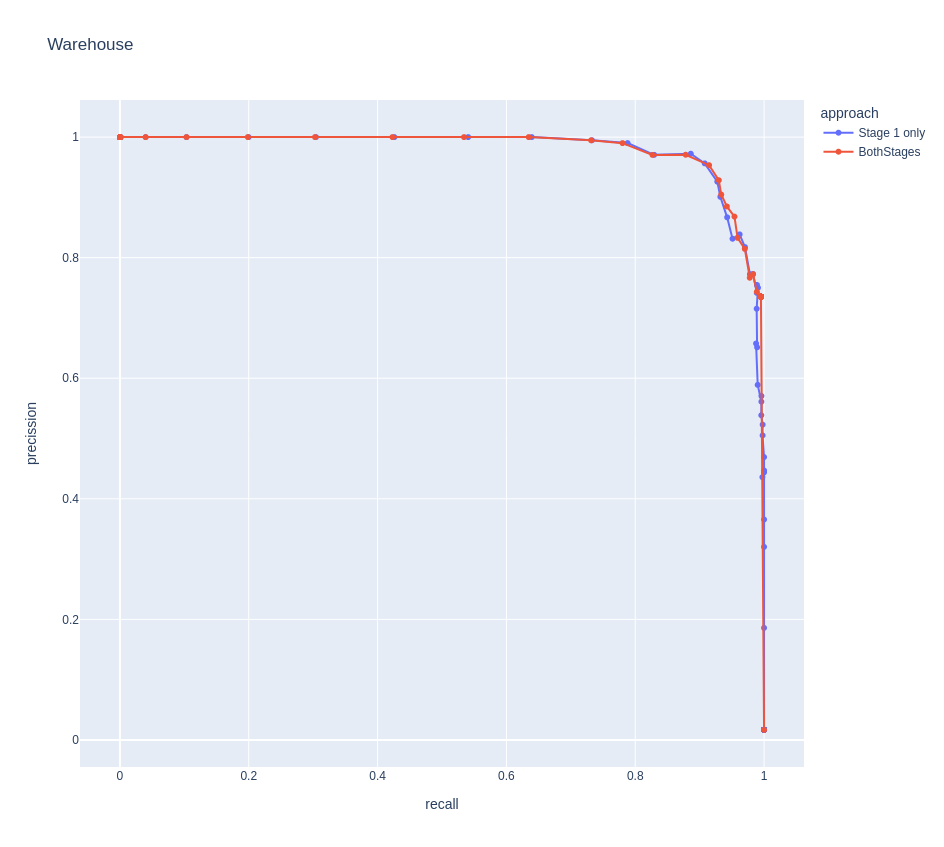
\includegraphics[height=0.3\textheight]{warehousePR.png}\label{fig:prCurvesWarehouse}}
    \hfill
    \subfloat[House environment]{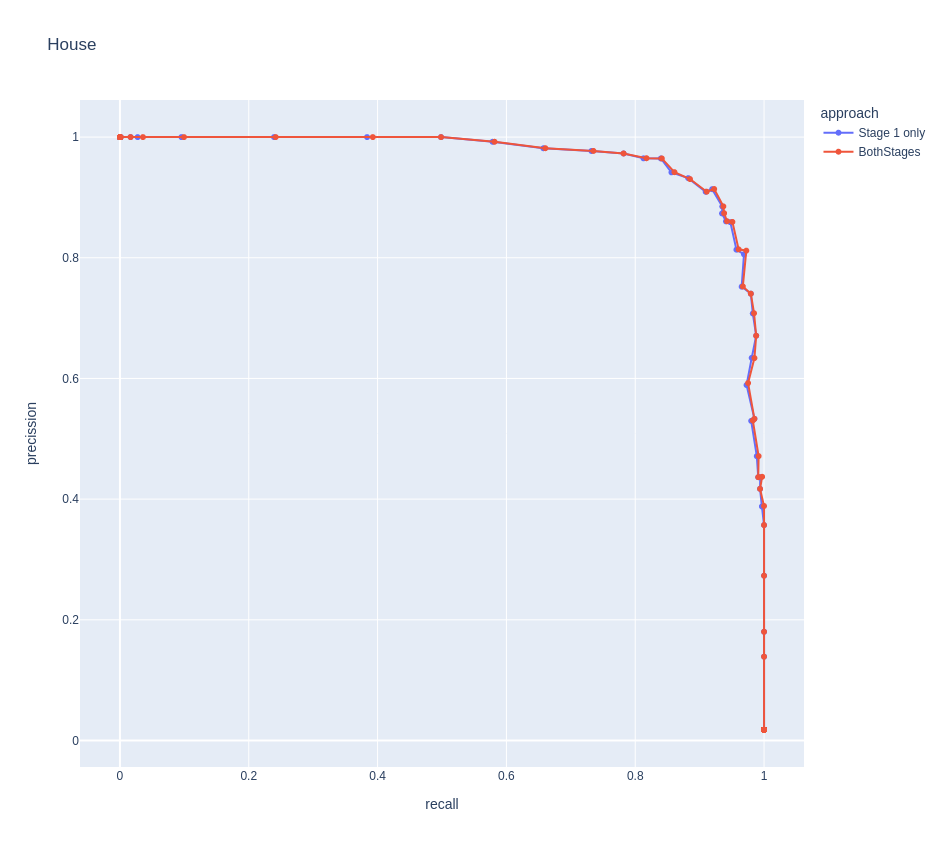
\includegraphics[height=0.3\textheight]{housePR.png}\label{fig:prCurveshouse}}
    \\
    \subfloat[Hospital environment]{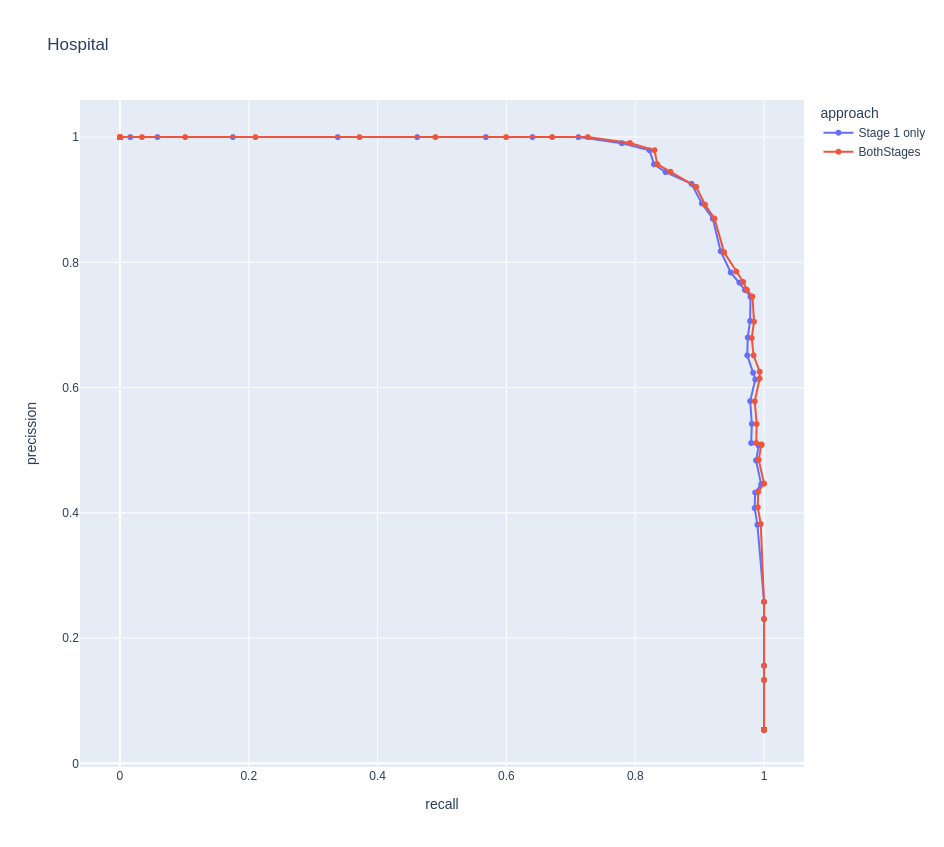
\includegraphics[height=0.3\textheight]{hospitalPR.png}\label{fig:prCurvesHospital}}
    \caption{PR Curves comparing Hierarchical and 2-Stage view matching approaches}
    \label{fig:prCurves}
\end{figure}


Because the thresholds influence only the LV matching part and not the LV building part, the local views were built and saved using the LV Dataset creator node, presented in section \ref{section:lvdatasetCreator}. This dataset was afterward used for evaluation instead of running the whole simulation, which saved a lot of time.\par
As Figure \ref{fig:prCurves} shows, both approaches have very similar results. Still, the method with two stages slightly outperforms the hierarchical approach with only the first stage by eliminating some false positive evaluations. Examples of false positives, evaluated by the first stage and eliminated by the second stage, are shown in Figure \ref{fig:eliminatedFPExamples}.\par

\begin{figure}[!tbp]
    \centering
    \subfloat{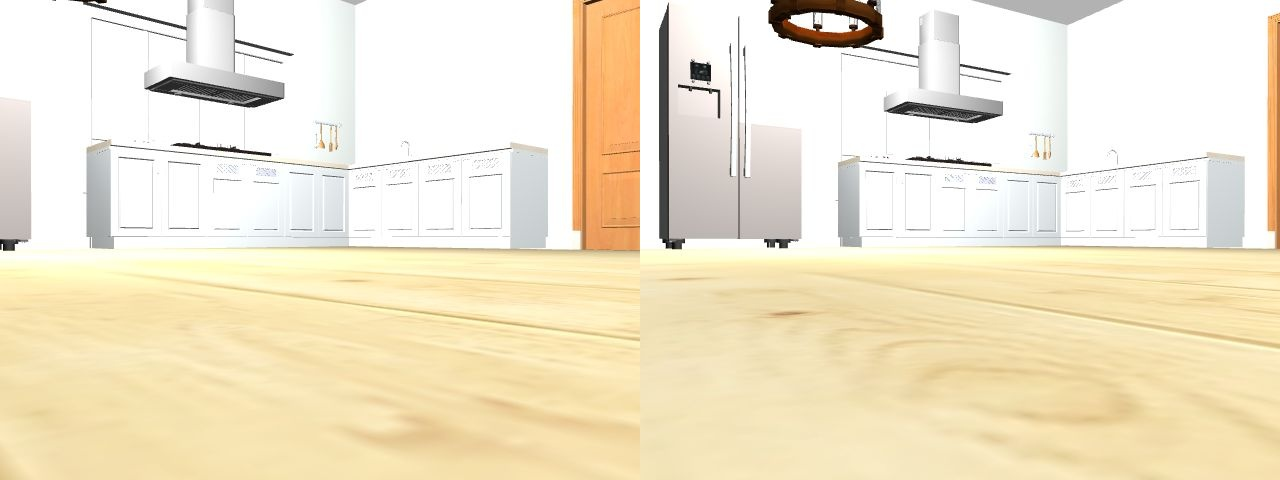
\includegraphics[width=0.8\textwidth]{eliminatedFPExample1.jpg}\label{fig:eFPEx1}}
    \\
    \subfloat{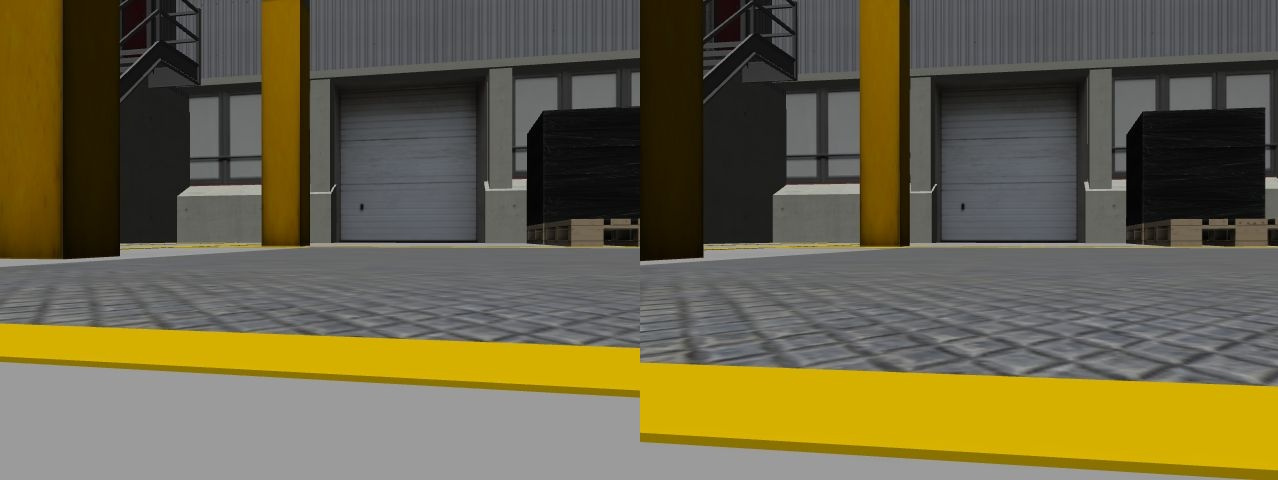
\includegraphics[width=0.8\textwidth]{eliminatedFPExample2.jpg}\label{fig:eFPEx2}}
    \caption{Examples of false positives eliminated by the second stage}
    \label{fig:eliminatedFPExamples}
\end{figure}

After the optimal thresholds were picked, the overall accuracy of both approaches was measured and compared with the accuracy of the visual place recognition used in the OpenRatSLAM. The results are shown in the table \ref{tab:accuracy}.

\begin{table}[htpb]
    \caption{Accuracy of all approaches in different environments}\label{tab:accuracy}
    \centering
    \begin{tabular}{l l l l}
        \toprule
        \textbf{}          & \textbf{1st stage only} & \textbf{both stages} & \textbf{OpenRatSLAM} \\
        \textbf{Warehouse} & 88.84 \%                & 89.28 \%             & 77.67 \%             \\
        \textbf{House}     & 86.69 \%                & 86.94 \%             & 41.25 \%             \\
        \textbf{Hospital}  & 86.19 \%                & 86.38 \%             & 79.36 \%             \\
        \bottomrule
    \end{tabular}
\end{table}

As the results show, both approaches have very similar results in all environments, but the method with both stages still slightly outperformed the technique with only the first stage. We can also see that both suggested approaches significantly outperformed the visual place recognition used in the OpenRatSLAM version in every environment, especially in the house world. Furthermore, the experiment results proved the ability to generalize on the environments diametrally different from the warehouse environment used for the model training.
